
\vspace{1cm}
{\let\clearpage\relax \chapter{Conclusioni}} 

Tenendo in considerazione la metrica MAPE sul validation set, il modello che ha mostrato i migliori risultati, è il KNN (che rimane pur sempre model-free), seguito dai modelli lineari. Questi ultimi non performano al meglio, ma questo può essere dovuto alla non corretta impostazione dei parametri (i resuidi dei modelli finali avrebbero potuto essere migliorati). L'aspettativa è quindi che il KNN si confermi il più preciso anche nella previsione del mese successivo.

\vspace{0.2cm}


\begin{table}[H]
    \centering
    \begin{tabular}{||c|c|c||} 
        \hline
        ARIMA & UCM & RNN \\ 
        \hline
        10.94\% & 11.13\% & 10.13\% \\
        \hline
    \end{tabular}
    \caption{Risultati del modello migliore per ogni categoria. }
\end{table}

\vspace{0.5cm}

In conclusione, i modelli vengono riaddestrati su tutta la serie storica a disposizione, in modo da effettuare una previsione sul mese di marzo 2005. 



\begin{figure}[H]
\centering
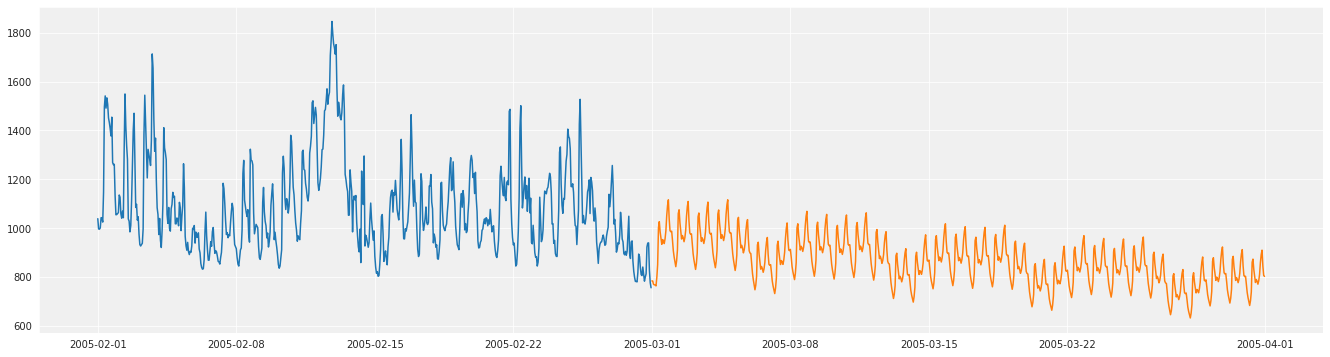
\includegraphics[width=14cm]{Pictures/prediction_marzo_arima.png}
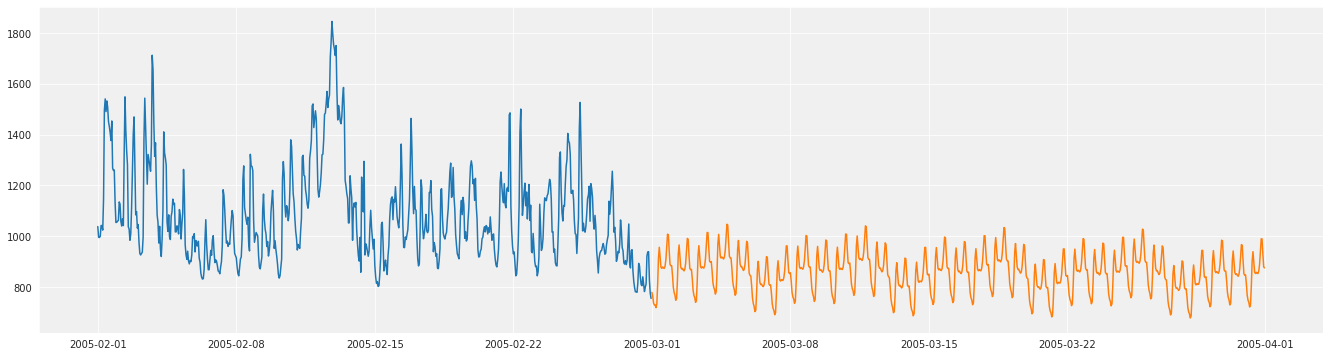
\includegraphics[width=14cm]{Pictures/prediction_marzo_ucm.png}
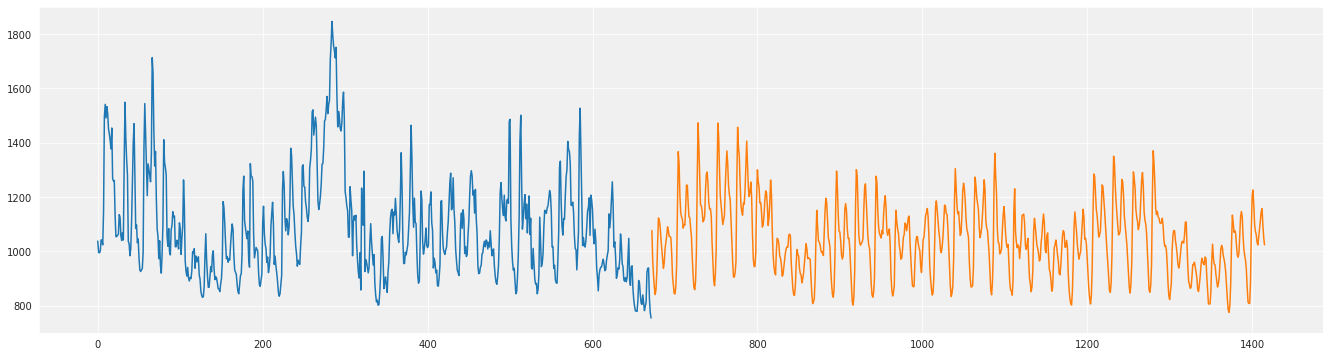
\includegraphics[width=14cm]{Pictures/prediction_marzo_knn.png}
\caption{Previsioni su marzo 2005 dei modelli ARIMA, UCM e KNN.}
\end{figure}